\label{sec:data-preparation}

Once the raw data was collected from trusted sources, it had to be cleaned, standardized, and transformed into a format suitable for both retrieval and generation. This phase shown in the Figure 5.3.1 plays a crucial role in ensuring the quality and efficiency of the RAG pipeline.

\subsection{Cleaning and Filtering}
\label{subsec:cleaning-filtering}

The raw textual data extracted from sources like WHO and CDC websites often contained a mix of useful content and noise. A cleaning pipeline was applied to ensure only relevant and high-quality information was retained.

\begin{itemize}
    \item \textbf{Structural Cleaning:} HTML content was parsed and converted into plain text while preserving logical sections (e.g., paragraphs, headers). This ensured the data remained well-structured for further processing.
    
    \item \textbf{Removal of Irrelevant Elements:} Common non-informative parts such as headers, footers, ads, navigation menus, and update timestamps were removed using pattern-matching and HTML parsing.
    
    \item \textbf{Redundancy Elimination:} Duplicate or repetitive information—like repeated titles or boilerplate disclaimers—was identified and removed. When similar content appeared multiple times, the most complete or contextually rich version was kept.
\end{itemize}

This process significantly improved the clarity and usefulness of the final dataset used in the RAG pipeline.

\subsection{Chunking}
\label{subsec:chunking}

Once the data was cleaned and filtered, the next crucial step involved splitting the text into coherent and manageable segments, a process known as chunking. This step is essential for the retrieval phase of the RAG (Retrieval-Augmented Generation) system because it enables the model to work with smaller, more focused passages instead of entire articles.

We applied a fixed-length token chunking strategy, where the textual content was segmented into chunks of 800 tokens each. To maintain contextual continuity across chunks and ensure that important information was not cut off at the edges, we used a sliding window approach with an overlap of 80 tokens between consecutive chunks. This overlapping approach allowed us to preserve the flow of ideas, especially when key information spanned across chunk boundaries.

Choosing 800 tokens as the chunk size provided a balance between depth of context and computational efficiency. Each chunk was large enough to capture meaningful information, such as a complete explanation of a symptom or a treatment recommendation, while still being short enough to work efficiently within the input limits of the language model.

These context-rich chunks formed the basic units for the embedding and retrieval process that powers the RAG system.

\subsection{Metadata Augmentation}
\label{subsec:metadata}

In addition to chunking the textual content, each chunk was enriched with metadata to enhance retrieval accuracy and provide additional context during query processing. The metadata included the source website (such as WHO, NIH, or CDC) and the document title from which the chunk was extracted.

This metadata helps the RAG system to better understand the origin and relevance of each chunk, allowing it to prioritize responses from trusted and authoritative sources. Moreover, having this contextual information supports clearer, more informative answers and makes it easier to trace back responses to their original documents for verification or updates.

\subsection{Embedding Generation}
\label{subsec:embeddings}

Following chunking, each text chunk was transformed into a dense vector representation using the \texttt{Bge-m3} embedding model. This model encodes the semantic meaning of text, enabling similarity comparisons between user queries and document chunks in a shared vector space.

Generating embeddings is a crucial step in preparing the data for retrieval, as it allows the system to identify and rank the most relevant information based on meaning rather than simple keyword overlap.

\subsection{Indexing in Vector Store}
\label{subsec:indexing}

After generating embeddings for all text chunks, they were indexed using ChromaDB, an efficient and open-source vector database. ChromaDB enables fast and accurate approximate nearest neighbor (ANN) searches based on vector similarity.

This indexing step plays a crucial role in the retrieval process, allowing the system to quickly identify and return the most relevant chunks in response to a user query. By organizing the vectorized data into an optimized structure, ChromaDB ensures low-latency performance during inference.

\begin{figure}[htbp]
  \centering
  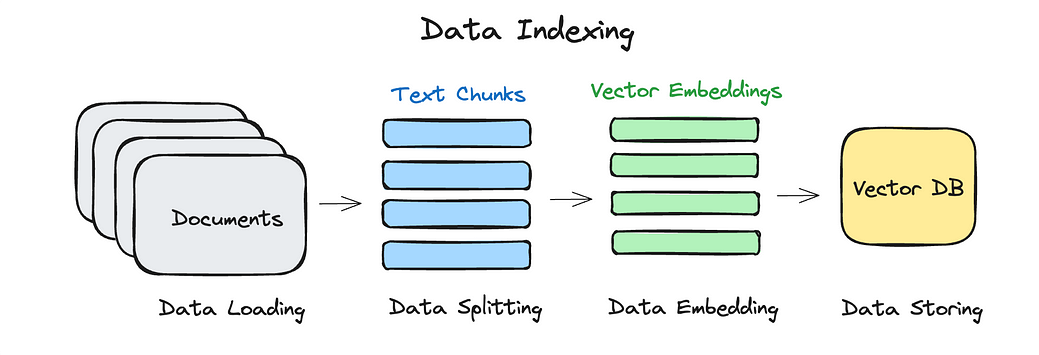
\includegraphics[width=0.8\textwidth]{images/Indexing_RAG.png}
  \caption{Indexing process} % Starred version
  \label{fig:indexing-process-manual}
\end{figure}

